\chapter{TÊN CHƯƠNG}

\noindent\textbf{Mục tiêu chương}

\noindent Nội dung này phải thể hiện rõ, sau khi hoàn thành chương học, người học có khả năng thực hiện những nhiệm vụ, yêu cầu chuyên môn hay vận dụng vào thực tiễn.

\noindent Kiến thức:

- Trình bày khái niệm, định nghĩa, thuật ngữ.

- Giải thích bản chất vấn đề.

- Hiểu rõ nguyên lý, quá trình hoạt động, vận hành.

- Phân tích, so sánh đối tượng, hiện tượng.

\noindent Kỹ năng: 

- Tính toán, phân tích số liệu.

- Thực hiện thao tác kỹ thuật hoặc mô phỏng.

\noindent Ứng dụng:

- Giải quyết bài tập hoặc tình huống thực tế.

\noindent Thái độ: 

- Có ý thức tuân thủ quy trình.

- Thể hiện tinh thần học tập nghiêm túc, trách nhiệm nghề nghiệp.

\section{Quy định biên soạn}
\hspace{0.5 cm}- Thông tư số 35/2021/TT-BGDĐT ngày 06 tháng 12 năm 2021 của Bộ Giáo dục và Đào tạo Quy định việc biên soạn, lựa chọn, thẩm định, duyệt và sử dụng tài liệu giảng dạy, giáo trình giáo dục đại học.

- Quyết định số 32/QĐ-ĐHGTVT ngày 03 tháng 4 năm 2023 của Hiệu trưởng Trường Đại học Giao thông vận tải Thành phố Hồ Chí Minh ban hành Quy định về việc biên soạn, lựa chọn, thẩm định, duyệt, xuất bản, in, phát hành và sử dụng tài liệu giảng dạy, giáo trình giáo dục đại học của Trường Đại học Giao thông vận tải Thành phố Hồ Chí Minh.

\section{Các yêu cầu đối với tài liệu kỹ thuật}
(1) Tài liệu kỹ thuật cần được thiết kế logic, khoa học, bám sát phạm vi dự án, cập nhật và phù hợp với mục tiêu vận hành của hệ thống.

\noindent (2) Nội dung không chỉ dừng ở việc nêu khái niệm, cần giải thích nguyên lý, phân tích và liên hệ ứng dụng kỹ thuật.

(3) Định dạng, cấu trúc và hình thức trình bày của tài liệu kỹ thuật cần đảm bảo tính đồng bộ, thống nhất, rõ ràng và dễ bảo trì. 

(4) Tài liệu kỹ thuật cần thường xuyên cập nhật khi hệ thống, tính năng, quy tắc nghiệp vụ, hoặc cách tính toán thay đổi để bảo đảm: Tính hiện đại, tính ứng dụng, tính thực tiễn.

(5) Tỷ lệ kiến thức có thể đáp ứng:

\hspace{0.5 cm}- 50 - 60% lý thuyết.

\hspace{0.5 cm}- 20 - 30% ví dụ thực tế.

\hspace{0.5 cm}- 10 - 20% bài tập thực hành.

(6) Tài liệu kỹ thuật cần cập nhật các tiến bộ của khoa học và công nghệ để bảo đảm:

\hspace{0.5 cm}- Tính hiện đại;

\hspace{0.5 cm}- Tính ứng dụng;

\hspace{0.5 cm}- Tính thực tiễn.

(7) Cần biên soạn tài liệu kỹ thuật theo cấu trúc sau:

\hspace{0.5 cm}1. Mục tiêu chương;

\hspace{0.5 cm}2. Nội dung kiến thức;

\hspace{0.5 cm}3. Ví dụ minh họa kỹ thuật;

\hspace{0.5 cm}4. Câu hỏi ôn tập;

\hspace{0.5 cm}5. Câu hỏi thảo luận;

\hspace{0.5 cm}6. Bài tập thực hành;

\hspace{0.5 cm}7. Tổng kết chương;

\hspace{0.5 cm}8. Đáp án, gợi ý trả lời câu hỏi ôn tập;

\hspace{0.5 cm}9. Phụ lục (nếu có);

\hspace{0.5 cm}10.Tài liệu tham khảo.

\section{Khổ giấy, lề trang}
- Khổ giấy: Khổ 19 cm x 27 cm.

- Lề trang giấy: Lề trên (Top): 2,0 cm; Lề dưới (Bottom): 2,0 cm; Lề trái (Left): 3,0 cm; Lề phải (Right): 2,0 cm. Chế độ hiển thị trang: Multiple pages: Mirror margin; Apply to: Whole document. Layout: Header: 1,27 cm; Footer: 1,27 cm. 
\section{Nội dung tài liệu kỹ thuật}
\subsection{Chương và tên Chương}
Tên chương có font chữ: Times New Roman. Kiểu chữ: In hoa, đậm. Cỡ chữ: 15. Khoảng cách với nội dung tài liệu: 16 pt. 
\subsection{Tiêu đề}
Font chữ: Times New Roman. Kiểu chữ: In đậm, chữ thường. Cỡ chữ: 12, cùng cỡ chữ với nội dung tài liệu. Khoảng cách giữa tiêu đề và nội dung tài liệu là 6 pt.
\subsection{Nội dung}
Nội dung tài liệu kỹ thuật trình bày thống nhất trong toàn bản thảo:

- Font chữ: Times New Roman. Kiểu chữ: Thường (Regular). 

- Cỡ chữ: 12. 

- Nội dung trình bày canh đều cả hai lề.

- Các đoạn văn cách nhau Spacing: Trước (Before): 6 pt; Sau (After): 6 pt.

- Chế độ giãn dòng: Line spacing - Single.

\subsection{Cách trình bày mục và tiểu mục}

Thống nhất cách trình bày mục và tiểu mục như sau:

\noindent\textbf{1.1 Tiêu đề 1}

\noindent\textbf{1.1.1 Tiêu đề 2}

\noindent\textbf{a. Tiêu đề 3}

\noindent\textbf{Tiêu đề 4}

\noindent\textit{Tiêu đề 5}

\noindent Tiêu đề 6:

\noindent\textbf{Lưu ý:} Không dùng tiểu mục 4 chữ số (Ví dụ: 1.1.1.1, 1.1.1.2, 1.1.1.3…), thay bằng các tiểu mục a, b, c… 

\section{Hình ảnh và bảng biểu}
\subsection{Hình ảnh, hình vẽ}

\begin{enumerate}[label=-]
	\item Số thứ tự của hình vẽ, hình ảnh theo chương, kiểu chữ in đậm. 
	\item Hình vẽ, hình ảnh trích từ tài liệu tham khảo, phải có nguồn trích dẫn và được diễn giải trong nội dung tài liệu, không trích dẫn ở cuối tên hình.
	\item Nếu hình vẽ, hình ảnh của tác giả thì không nêu nguồn trích dẫn.
	\item Tất cả hình ảnh cần được đề cập, giải thích, diễn giải trong nội dung tài liệu.
\end{enumerate}

\noindent Ví dụ:

\noindent Cảm biến dòng xoáy ứng dụng nhiều trong các lĩnh vực yêu cầu đo lường không tiếp xúc như đo độ rung, khoảng cách và kiểm tra bề mặt vật liệu. Cảm biến dòng xoáy bao gồm một đầu dò chứa cuộn dây (Hình \ref {fig:hinh1_1})  được kích tại tần số cao, khoảng 1 MHz \cite{ref1}.

\begin{figure}[h]
	\centering
	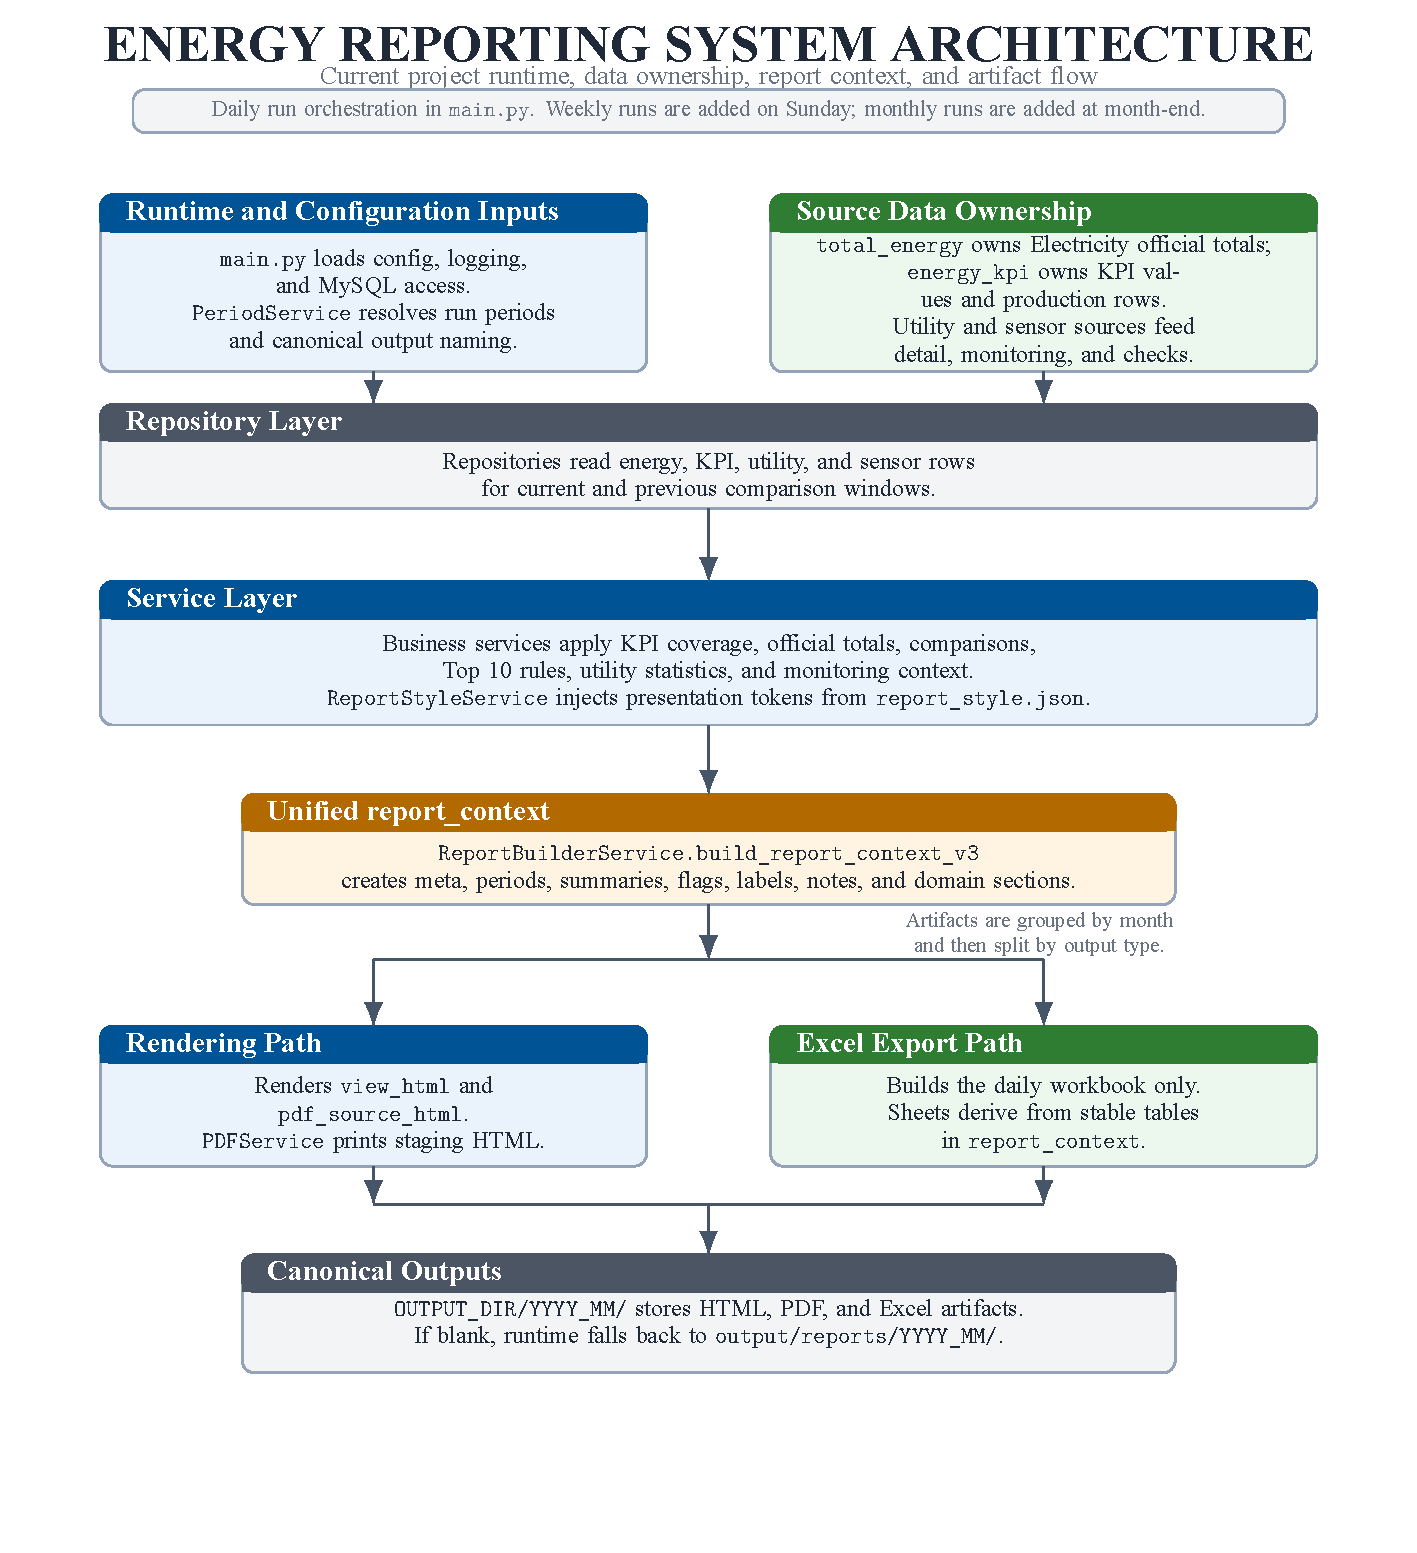
\includegraphics[width=0.8\textwidth]{figure/hinh1_1}
	\caption{Hình minh họa có tham khảo nguồn trích dẫn}
	\label{fig:hinh1_1}
\end{figure}

\noindent Trước khi bơm làm việc, thân bơm và ống hút được điền đầy chất lỏng. Khi bơm làm việc, bánh công tác quay, các phần tử chất lỏng tại bánh công tác dưới ảnh hưởng của lực ly tâm dồn từ trong ra ngoài, chuyển động theo máng dẫn và đi vào ống đẩy với áp suất cao hơn, đó là quá trình đẩy (Hình \ref{fig:hinh1_2}) \cite{ref2}.

\begin{figure}[h]
	\centering
	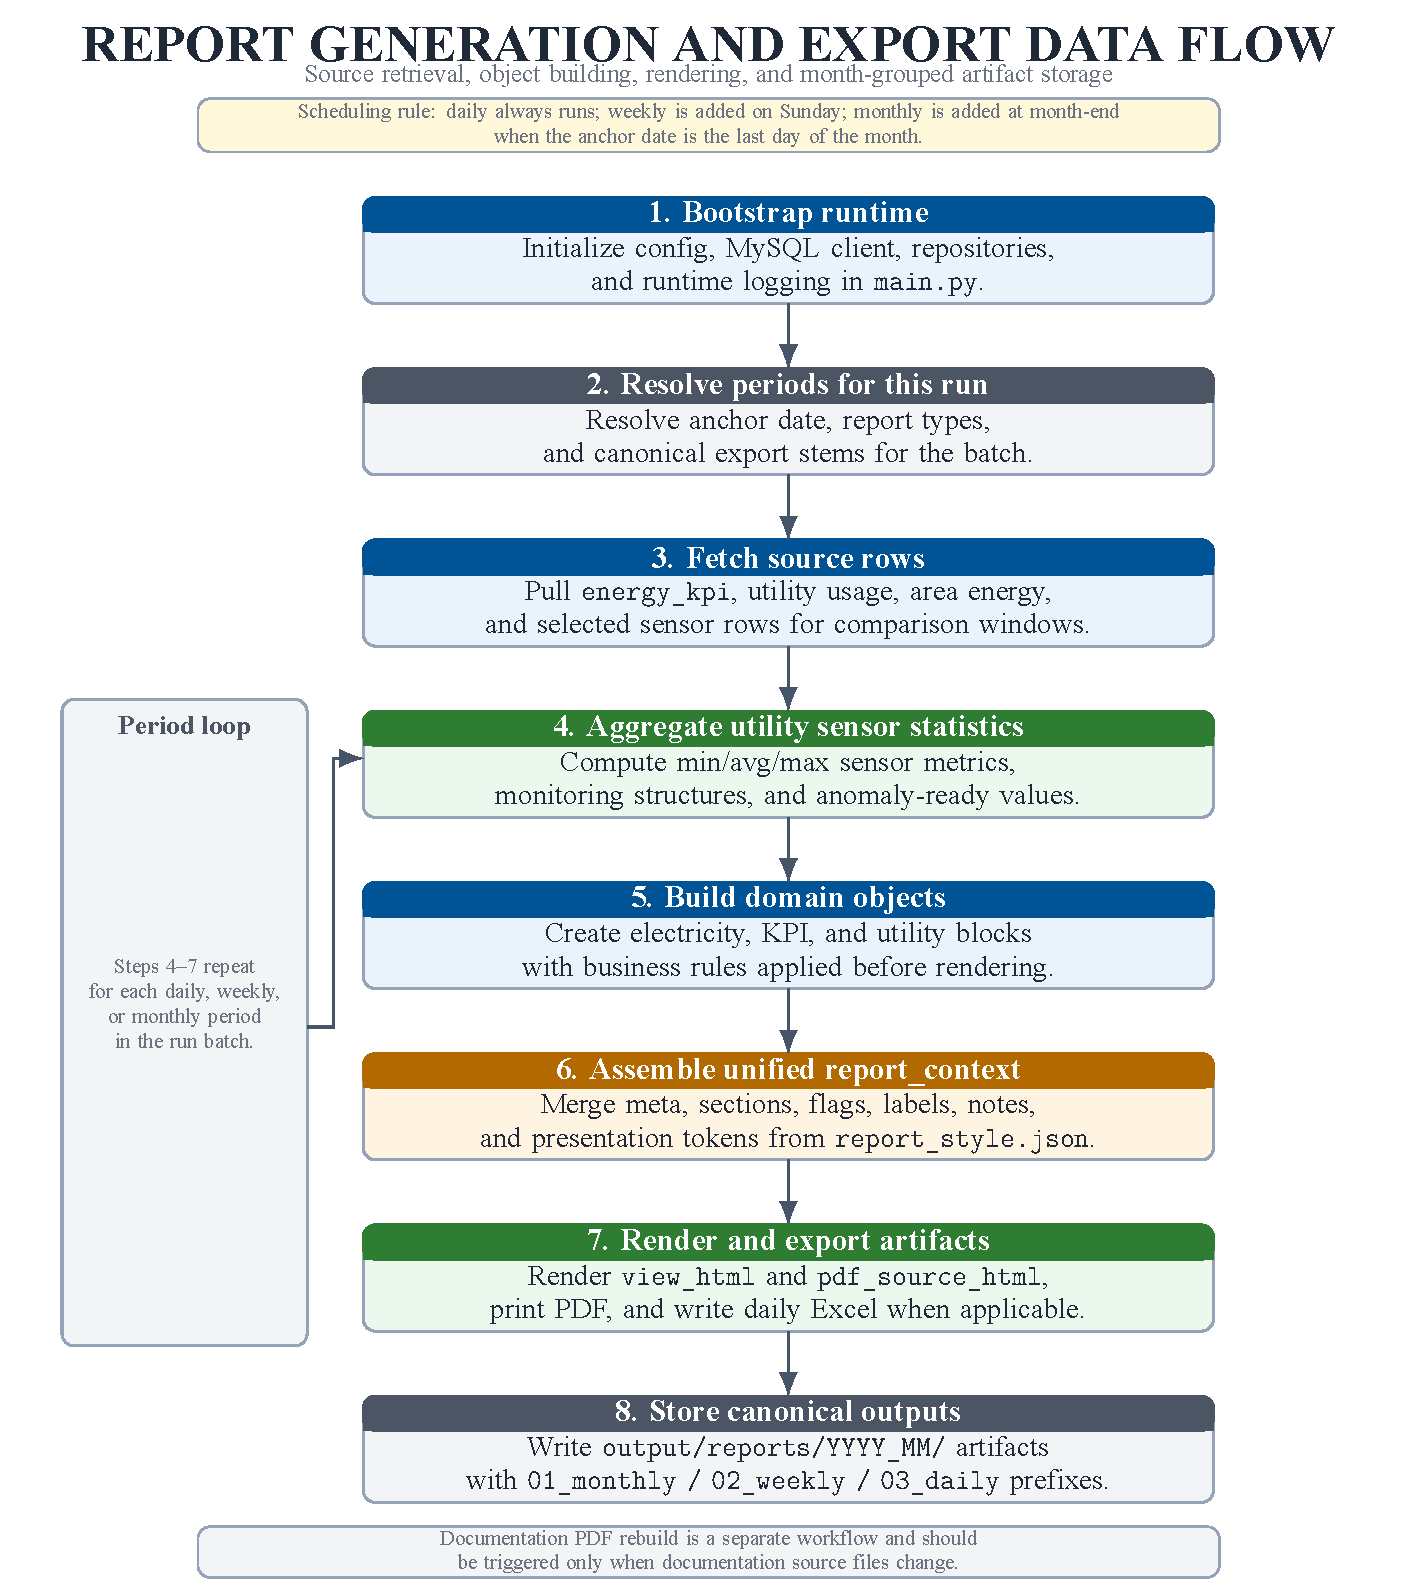
\includegraphics[width=0.8\textwidth]{figure/hinh1_2}
	
	\textit{(1) Bánh công tác; (2) Trục bơm; (3) Bộ phận dẫn hướng vào; 
		(4) Bộ phận dẫn hướng ra (buồng xoắn ốc); (5) Ống hút; (6) Ống đẩy}
	\caption{Hình minh họa có tham khảo nguồn trích dẫn}
	\label{fig:hinh1_2}
	\end{figure}
	
\subsection{Bảng biểu}
\begin{enumerate}[label=-]
	 \item Số thứ tự bảng biểu theo Chương.
	 \item Bảng biểu trích từ tài liệu tham khảo, phải có nguồn trích dẫn và được diễn giải trong nội dung tài liệu, không trích dẫn ở cuối tên bảng.
	 \item Nếu bảng biểu của tác giả thì không nêu nguồn trích dẫn.
	 \item Tất cả bảng biểu cần được đề cập, giải thích, diễn giải trong nội dung tài liệu.
\end{enumerate} 

\noindent Ví dụ:
\begin{table}[h]
	\centering
	\renewcommand{\arraystretch}{1.3}
	\caption{Bảng minh họa có tham khảo nguồn trích dẫn}
	\label{tab:Bang1_1}
	\begin{tabularx}{\linewidth}{|
		>{\centering\arraybackslash}p{3cm}|
		>{\centering\arraybackslash}X|	
		>{\centering\arraybackslash}X|
		>{\centering\arraybackslash}X|}
		\hline
		\textbf{Loại cảm biến điện dung} &
		\textbf{Nguyên lý hoạt động} &
		\textbf{Ứng dụng} &
		\textbf{Đặc điểm} \\
		\hline
		Cảm biến tiệm cận điện dung &
		Thay đổi điện dung khi vật thể đến gần bề mặt cảm biến &
		Phát hiện đối tượng trong công nghiệp, tự động &
		Nhạy với vật liệu dẫn điện và không dẫn điện \\
		\hline
		Cảm biến vị trí điện dung &
		Đo sự thay đổi điện dung giữa hai bề mặt song song khi khoảng cách đổi &
		Đo vị trí chính xác trong máy CNC, hệ thống kiểm tra &
		Độ phân giải cao, phù hợp với đo vị trí nhỏ \\
		\hline
	\end{tabularx}
\end{table}

\noindent Các loại cảm biến điện dung phổ biến hiện nay rất đa dạng, Bảng \ref{tab:Bang1_1}  \cite{ref3} tổng hợp phân loại dựa trên nguyên lý hoạt động, ứng dụng và đặc điểm của chúng.

\section{Công thức, phương trình}
Tất cả công thức, phương trình đều đánh số thứ tự, theo chương; thống nhất font chữ, kiểu chữ, cỡ chữ trong toàn bản thảo.\\
Ví dụ:\\
Công thức \ref{eq:eq1} tính độ tự cảm của một cuộn dây trong điện từ học:
\begin{equation}
	L=\frac{\mu N^2 A}{l}
	\label{eq:eq1}
\end{equation}
Trong đó:\\
\begin{tabular}{p{0.5 cm}ll}
	& $\mu$ &: Độ từ thẩm của vật liệu từ;\\
	& $N$ &: Số vòng dây;\\
	& $A$ &: Diện tích mặt cắt;\\
	& $l$ &: Chiều dài của lõi từ tính.\\
\end{tabular}
\section{Ví dụ minh họa}
Ví dụ minh họa giúp người học hiểu cách áp dụng lý thuyết vào thực tế kỹ thuật. Chẳng hạn:

- Case study kỹ thuật;

- Hệ thống công nghiệp thực tế;

- Mô phỏng kỹ thuật;

- …

\section{Câu hỏi thảo luận, bài tập thực hành}

Phần này có thể trải đều toàn chương. Trong đó:

\noindent\textbf{Câu hỏi thảo luận}

\noindent Nhằm giúp người học phát triển tư duy phản biện, phân tích vấn đề, nâng cao kỹ năng làm việc nhóm.

\noindent\textbf{Bài tập thực hành}

\noindent Để người học áp dụng kiến thức vào hệ thống kỹ thuật thực tế.

\section{Tổng kết Chương 1}

Nội dung này tổng hợp và hệ thống hóa những kiến thức trọng tâm của chương, qua đó giúp người học củng cố và hệ thống hóa kiến thức đã học.

% ================== BÀI TẬP CHƯƠNG 1 ==================
\newpage

\section*{}
\begin{center}
	\bfseries\fontsize{12}{14}\selectfont
	Câu hỏi ôn tập Chương 1
\end{center}
\addcontentsline{toc}{section}{Câu hỏi ôn tập Chương 1}

\noindent\textbf{Câu 1.} Nội dung câu hỏi tự luận

\noindent\textbf{Câu 2.} Nội dung câu hỏi tự luận

\noindent\textbf{Câu 6.} Nội dung câu hỏi
\begin{enumerate}[label=\Alph*.]
\item Nội dung đáp án
\item Nội dung đáp án
\item Nội dung đáp án
\item Nội dung đáp án
\end{enumerate}
...\\
\noindent\textbf{Câu 30.} Nội dung câu hỏi
\begin{enumerate}[label=\Alph*.]
\item Nội dung đáp án
\item Nội dung đáp án
\item Nội dung đáp án
\item Nội dung đáp án
\end{enumerate}
...\\
\noindent\textbf{Lưu ý:}

- Câu hỏi ôn tập nhằm hỗ trợ người học có thể kiểm tra mức độ hiểu bài, hệ thống lại kiến thức, chuẩn bị cho kiểm tra hoặc thi.

- Câu hỏi ôn tập biên soạn theo Quy định về việc xây dựng, đánh giá chất lượng và quản lý ngân hàng câu hỏi thi trắc nghiệm khách quan nhiều lựa chọn (Ban hành kèm theo Quyết định số 675/QĐ-ĐHGTVT ngày 27 tháng 9 năm 2021 của Hiệu trưởng Trường Đại học Giao thông vận tải Thành phố Hồ Chí Minh).

- Kết thúc mỗi chương có \textbf{tối thiểu 30 câu hỏi, bài tập ôn tập}. Chia các câu hỏi  thành các gói (tự luận, trắc nghiệm) khác nhau đáp ứng chuẩn đầu ra.


% ================== ĐÁP ÁN, GỢI Ý TRẢ LỜI CÂU HỎI ÔN TẬP ==================
\newpage
\section*{}
\begin{center}
	\bfseries\fontsize{15}{14}\selectfont
	ĐÁP ÁN, GỢI Ý TRẢ LỜI CÂU HỎI ÔN TẬP
\end{center}

\noindent\textbf{CHƯƠNG 1.}

\noindent\textbf{Câu 1.} Nội dung gợi ý trả lời (Hướng dẫn trả lời chi tiết, không hướng dẫn theo kiểu chung là Tham khảo mục).

\noindent\textbf{Câu 2.} Nội dung gợi ý trả lời (Hướng dẫn trả lời chi tiết, không hướng dẫn theo kiểu chung là Tham khảo mục).

.....

\noindent\textbf{Câu 6.} A

.....

\noindent\textbf{Câu 30.} B

.....

% ================== PHỤ LỤC ==================
\newpage
\section*{}
\begin{center}
	\bfseries\fontsize{15}{14}\selectfont
	PHỤ LỤC
\end{center}

Tác giả/Nhóm tác giả trình bày phụ lục tại mục này (nếu có).